\graphicspath{
    {figures_and_references/urban_surface_detection/}
    {figures_and_references/footprints_paper/}
    {figures_and_references/EELISA_conference/}
    {figures_and_references/fragility_curves/}
}

% \selectlanguage{english}
\renewcommand{\chapternametext}{Chapter \thechapter: Capacity curve generation with machine learning}

\begin{refsection}

\chapter{\chapternametext}
\

\renewcommand{\headingtextL}{}
\renewcommand{\headingtextR}{\chapternametext}
\begingroup
 \flushbottom
 \setlength{\parskip}{0pt plus 1fil}%
 \localtableofcontents 
\endgroup

\begingroup
 \flushbottom
 \setlength{\parskip}{0pt plus 1fil}%
 \locallistoffigures
\endgroup


\newpage

\setcounter{section}{0} 



\FloatBarrier

\renewcommand{\sectionnametext}{Introduction}
\renewcommand{\headingtextL}{\chapternametext}
\renewcommand{\headingtextR}{\thesection. \sectionnametext}
\section{\sectionnametext}


Traditional vulnerability assessments typically assign generic capacity curves from existing building taxonomies to represent regional building stocks \footcite{yepes-estrada_modeling_2017,barbat_seismic_2010}. While this approach provides a practical basis for large-scale analyses, it often fails to capture the structural variability present in heterogeneous and informal urban environments. As discussed in Chapter 1, broad typological classes can be identified, but the seismic response of an individual building remains highly dependent on a combination of geometric and structural characteristics, including the number of storeys, eccentricity ratios, confinement conditions, and other parameters that vary from one structure to another.

Alongside the research presented in this thesis, the author developed three Python packages that support different stages of the proposed workflow. These packages are openly available through GitHub and have been used throughout the implementation of the methodology described in the following sections.

\renewcommand{\sectionnametext}{Automated FEM dataset generation}
\renewcommand{\headingtextR}{\thesection. \sectionnametext}
\section{\sectionnametext}

To generate a representative training dataset, an automated finite element modelling workflow was developed by other members of the research team using the open-source software \textit{OpenSees}. Instead of manually creating individual structural models, a parametric generator was created to automatically produce idealized aggregates consisting of up to five contiguous units. This row-house configuration reflects the dense urban fabric commonly observed in many of the pilot regions and is representative of the building typologies frequently encountered in seismic exposure studies \footcite{yepes-estrada_modeling_2017}.

\subsection{Parametric structural variations}

\begin{figure}[htbp]
    \centering
    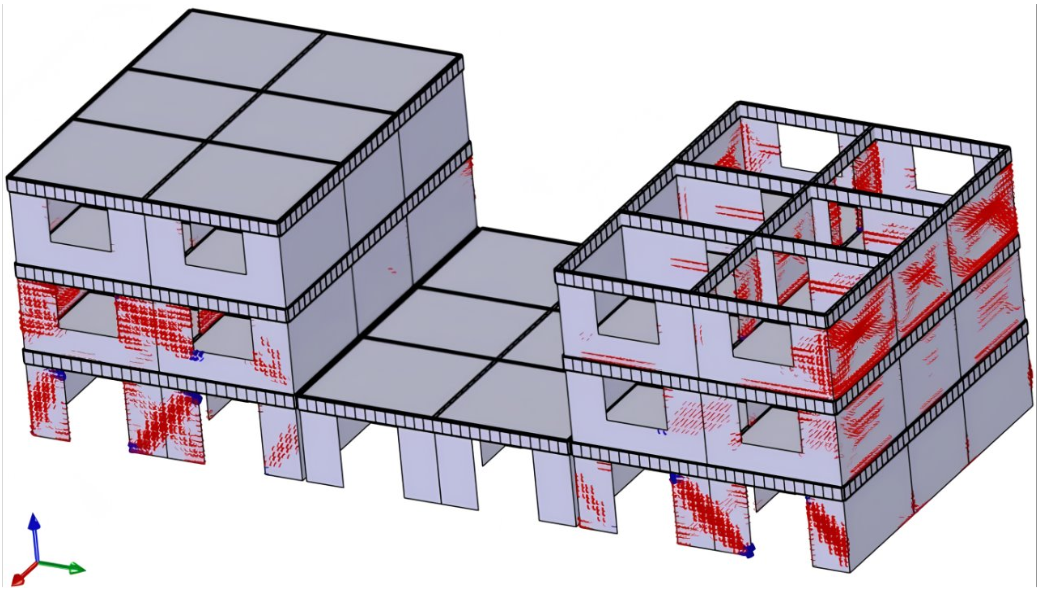
\includegraphics[width=0.6\linewidth]{figures/buildings_simulation.png}
    \caption{Example of a building row with 3 buildings and different number of floors.}
    \label{fig:FEM}
\end{figure}

The generator explores the design space by systematically varying a set of key engineering parameters depending on the configurations required to train the machine learning model (fig. \ref{fig:FEM}). Internal wall configurations are modified to produce different levels of eccentricity between the centre of mass and the centre of stiffness, introducing varying degrees of geometric and mass irregularity. The number of storeys and the street slope are also adjusted to represent realistic topographic conditions and differences in building height. In addition, the modelling framework considers both rigid and flexible diaphragm assumptions, allowing different floor-to-wall connection behaviours to be represented. Material properties are treated as stochastic variables, enabling the dataset to capture the influence of local variations in strength and ductility on the overall structural response.

By automating these variations, a large dataset covering a broad range of nonlinear responses can be generated efficiently (fig. \ref{fig:curves_rel_pos}). Rather than relying on case-specific modelling, the machine learning model learns a continuous relationship between geometric descriptors and the resulting force--displacement behaviour.

\begin{figure}[htbp]
    \centering
    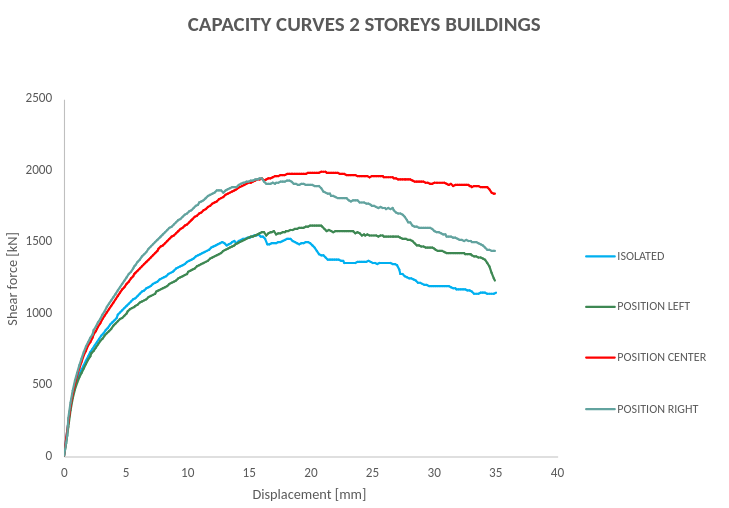
\includegraphics[width=0.6\linewidth]{figures/capacity_curve_1.png}
    \caption{Three different capacity curves obtained from the simulation by changing the relative position of the building within the row.}
    \label{fig:curves_rel_pos}
\end{figure}


\renewcommand{\sectionnametext}{Surrogate modelling via gaussian process regression}
\renewcommand{\headingtextR}{\thesection. \sectionnametext}
\section{\sectionnametext}

The computational cost of nonlinear static pushover analyses makes it impractical to simulate every structure within a city-scale building inventory. To overcome this limitation, a surrogate modelling framework based on Gaussian Process Regression (GPR) is adopted, providing rapid predictions of structural capacity while retaining information about model uncertainty \footcite{rasmussen2003gaussian}.

\subsection{Framework and uncertainty quantification}

To represent the high-dimensional output of pushover analyses efficiently, Principal Component Analysis (PCA) is combined with GPR. PCA projects the capacity curves into a reduced latent space, capturing the dominant patterns of structural behaviour while reducing the dimensionality of the learning problem.

A key advantage of GPR is its Bayesian formulation \footcite{rasmussen2003gaussian}. For each prediction, the model provides both a mean estimate ($\mu_*$) and an associated variance ($\sigma_*^2$). When the model encounters building configurations that are poorly represented in the training dataset, the predicted uncertainty increases, providing a direct indication of reduced confidence in the estimated response (fig. \ref{fig:gpr_curve_example}). This information can be used to identify underrepresented regions of the parameter space and guide the generation of additional FEM simulations.

To avoid unconservative estimates of structural resistance, a conservative bias factor of 0.05 is incorporated into the regression process. This adjustment shifts the predicted capacities toward slightly lower values, reducing the risk of overestimating building performance and improving the robustness of the resulting fragility models.

\begin{figure}[htbp]
    \centering
    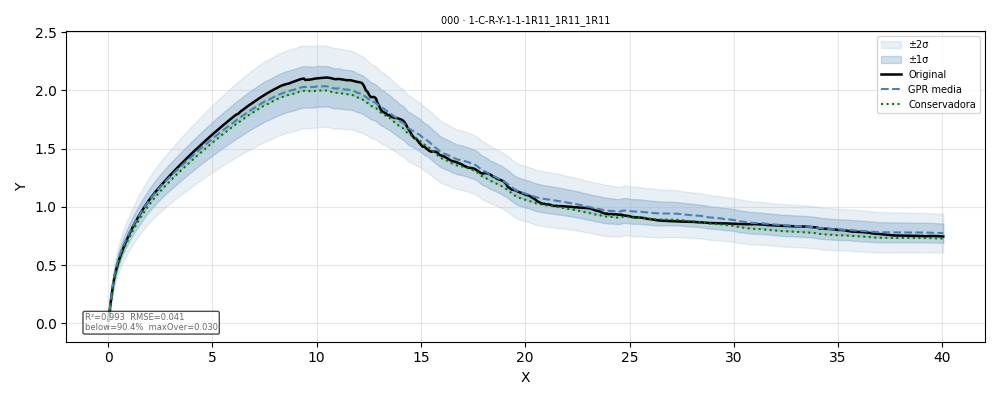
\includegraphics[width=\linewidth]{figures/example_curve.png}
    \caption{One example of a capacity curve output by the GPR model.}
    \label{fig:gpr_curve_example}
\end{figure}



\renewcommand{\sectionnametext}{Fragility curve framework}
\renewcommand{\headingtextR}{\thesection. \sectionnametext}
\section{\sectionnametext}

The final output of the proposed methodology is a set of seismic fragility curves. Fragility functions express the conditional probability of a building reaching or exceeding a specific damage state for a given level of seismic demand and constitute one of the most widely used tools in probabilistic seismic risk assessment \footcite{barbat_seismic_2010,mouroux_presentation_2006}. In contrast to approaches that assign predefined vulnerability functions to broad building classes, the framework developed in this thesis generates building-specific fragility curves by combining machine-learning-based capacity predictions with explicit uncertainty quantification.

\subsection{Probabilistic definition}

Fragility curves are represented using a lognormal cumulative distribution function, following common practice in earthquake engineering \footcite{milutinovic_wp4_2003,jimenez-martinez_methodology_2024}:

\begin{equation}
    P(ds \geq DS_i \mid S_d) =
    \Phi \left[
    \frac{\ln(S_d/\bar{S}_{d,ds})}
    {\beta_{ds}}
    \right]
\end{equation}

where $\bar{S}_{d,ds}$ denotes the median spectral displacement associated with damage state $DS_i$, $\beta_{ds}$ is the logarithmic standard deviation describing the uncertainty of the fragility function, and $\Phi$ represents the standard normal cumulative distribution function.

\subsection{Uncertainty propagation and integration}

One of the main advantages of the proposed methodology is the ability to propagate uncertainty throughout the entire workflow, from remote sensing observations to structural response prediction. The total uncertainty associated with each fragility function is expressed as

\begin{equation}
    \beta_{ds}=
    \sqrt{
    \beta_{capacity}^{2}
    +
    \beta_{demand}^{2}
    +
    \beta_{method}^{2}
    }.
\end{equation}

The capacity uncertainty, $\beta_{capacity}$, incorporates both epistemic and aleatory sources. The epistemic component originates from the Gaussian Process Regression surrogate model, which provides a predictive variance ($\sigma_*^2$) together with the mean capacity estimate \footcite{rasmussen2003gaussian}. This variance reflects the confidence of the model in regions of the parameter space that may be underrepresented in the training dataset. Additional aleatory variability is introduced through stochastic material properties, accounting for the natural dispersion in masonry and concrete strengths observed in local construction practices.

The demand uncertainty, $\beta_{demand}$, captures the inherent variability of earthquake ground motion, including differences in intensity and spectral shape between events. Finally, the methodological uncertainty, $\beta_{method}$, accounts for simplifications introduced by the remote-sensing-based exposure model, including the representation of complex structures through footprint-derived geometric proxies and simplified structural idealizations.

\subsection{Integrated workflow}

The proposed framework operates as a fully automated pipeline linking remote sensing observations with seismic risk metrics.

The process begins with the extraction of building footprints from high-resolution aerial or satellite imagery using fine-tuned deep-learning models, including Mask2Former and SAM2. Geometric descriptors and material-related proxies are subsequently derived using the \textit{SeismicBuildingExposure} package, one of three Python packages developed as part of this thesis and made publicly available through GitHub. Together, these tools provide parameters such as building dimensions, slenderness, eccentricity, compactness, and typological indicators inferred from geospatial information.

These descriptors are then supplied to the GPR surrogate model, which predicts the corresponding capacity curve while simultaneously providing an estimate of predictive uncertainty. The use of Gaussian Processes is particularly advantageous because it naturally produces probabilistic predictions rather than deterministic outputs \footcite{rasmussen2003gaussian}. Multiple realizations of the capacity curve can therefore be generated by sampling from the posterior distribution of the model.

The resulting ensemble of capacity curves is transformed into the ADRS (Acceleration--Displacement Response Spectrum) format and combined with damage-state thresholds to derive fragility functions. By integrating uncertainties associated with structural capacity, seismic demand, material variability, and methodological assumptions, the final fragility curves provide a probabilistic representation of seismic performance rather than a single deterministic estimate. This allows decision-makers to evaluate both expected risk and associated confidence levels, supporting more robust urban resilience and disaster-risk-reduction strategies.

The proposed approach addresses a key limitation of conventional vulnerability assessments, namely the reliance on generic capacity curves assigned to broad building classes \footcite{yepes-estrada_modeling_2017}. Instead, fragility functions are generated directly from measurable building characteristics extracted from remote sensing data, enabling scalable and spatially consistent seismic risk assessments across large urban areas.

\FloatBarrier

\newpage

\renewcommand{\sectionnametext}{References}
\renewcommand{\headingtextR}{\thesection. \sectionnametext}
\section{\sectionnametext}
\printbibliography[heading=none]

\end{refsection}